\documentclass{article}

\usepackage[utf8]{inputenc}
\usepackage[margin=1in]{geometry}
\usepackage{pgfplots}
%\usepgfplotslibrary{plotmarks}

\usepackage{pdflscape}

\usepackage{float}
\usepackage{subcaption}


%for units
\usepackage[binary-units=true]{siunitx}

\title{test plots}
\author{callum.iddon }
\date{April 2017}

\begin{document}

\maketitle

\section{Introduction}

HELLO! \SI{9.70}{\micro\second}

\newlength\figureheight
\newlength\figurewidth
\setlength\figureheight{7cm}
\setlength\figurewidth{\textwidth}
\input{test.tex}

\begin{landscape}
 \begin{figure}[H]
    \centering
    \begin{subfigure}{\textwidth}
      \centering
        % This file was created by matplotlib2tikz v0.6.6.
\begin{tikzpicture}

\definecolor{color1}{rgb}{0,0.75,0.75}
\definecolor{color0}{rgb}{0.75,0,0.75}

\begin{axis}[
title={Bandwidth for Message Size 1024B},
ylabel={Bandwidth \si{\mega\byte\per\second}},
xmin=-1.74875, xmax=12.38625,
ymin=6.22565964057004, ymax=3671.30381671607,
ymode=log,
width=\figurewidth,
height=\figureheight,
xtick={-0.68125,0.31875,1.31875,2.31875,3.31875,4.31875,5.31875,6.31875,7.31875,8.31875,9.31875,10.31875,11.31875},
xticklabels={Cloud,scarf10,scarf11,scarf12,scarf13,scarf14,scarf15,scarf16,broadwell256G,haswell256G,ivybridge128G,ivybridge2000G,ivybridge512G},
ytick={0.1,1,10,100,1000,10000,100000},
yticklabels={,,${10^{1}}$,${10^{2}}$,${10^{3}}$,,},
tick align=outside,
xticklabel style = {rotate=60},
xmajorticks=false,
ytick pos=left,
x grid style={lightgray!92.026143790849673!black},
y grid style={lightgray!92.026143790849673!black},
legend style={at={(0.97,0.03)}, anchor=south east, draw=white!80.0!black},
legend entries={{IBV},{SHM-2},{SHM-1},{TCP}},
legend cell align={left}
]
\addlegendimage{ybar,ybar legend,fill=blue,draw opacity=0};
\draw[fill=blue,draw opacity=0] (axis cs:-1.10625,0) rectangle (axis cs:-0.89375,0);
\draw[fill=blue,draw opacity=0] (axis cs:-0.10625,0) rectangle (axis cs:0.10625,109.432);
\draw[fill=blue,draw opacity=0] (axis cs:0.89375,0) rectangle (axis cs:1.10625,225.258);
\draw[fill=blue,draw opacity=0] (axis cs:1.89375,0) rectangle (axis cs:2.10625,234.966);
\draw[fill=blue,draw opacity=0] (axis cs:2.89375,0) rectangle (axis cs:3.10625,123.09);
\draw[fill=blue,draw opacity=0] (axis cs:3.89375,0) rectangle (axis cs:4.10625,154.324);
\draw[fill=blue,draw opacity=0] (axis cs:4.89375,0) rectangle (axis cs:5.10625,243.07);
\draw[fill=blue,draw opacity=0] (axis cs:5.89375,0) rectangle (axis cs:6.10625,278.32);
\draw[fill=blue,draw opacity=0] (axis cs:6.89375,0) rectangle (axis cs:7.10625,0);
\draw[fill=blue,draw opacity=0] (axis cs:7.89375,0) rectangle (axis cs:8.10625,0);
\draw[fill=blue,draw opacity=0] (axis cs:8.89375,0) rectangle (axis cs:9.10625,0);
\draw[fill=blue,draw opacity=0] (axis cs:9.89375,0) rectangle (axis cs:10.10625,0);
\draw[fill=blue,draw opacity=0] (axis cs:10.89375,0) rectangle (axis cs:11.10625,0);
\addlegendimage{ybar,ybar legend,fill=color0,draw opacity=0};
\draw[fill=color0,draw opacity=0] (axis cs:-0.89375,0) rectangle (axis cs:-0.68125,1086.00966666667);
\draw[fill=color0,draw opacity=0] (axis cs:0.10625,0) rectangle (axis cs:0.31875,1132.614);
\draw[fill=color0,draw opacity=0] (axis cs:1.10625,0) rectangle (axis cs:1.31875,1318.348);
\draw[fill=color0,draw opacity=0] (axis cs:2.10625,0) rectangle (axis cs:2.31875,1355.988);
\draw[fill=color0,draw opacity=0] (axis cs:3.10625,0) rectangle (axis cs:3.31875,995.168);
\draw[fill=color0,draw opacity=0] (axis cs:4.10625,0) rectangle (axis cs:4.31875,1058.894);
\draw[fill=color0,draw opacity=0] (axis cs:5.10625,0) rectangle (axis cs:5.31875,927.456);
\draw[fill=color0,draw opacity=0] (axis cs:6.10625,0) rectangle (axis cs:6.31875,942.358);
\draw[fill=color0,draw opacity=0] (axis cs:7.10625,0) rectangle (axis cs:7.31875,1263.688);
\draw[fill=color0,draw opacity=0] (axis cs:8.10625,0) rectangle (axis cs:8.31875,975.5);
\draw[fill=color0,draw opacity=0] (axis cs:9.10625,0) rectangle (axis cs:9.31875,1127.324);
\draw[fill=color0,draw opacity=0] (axis cs:10.10625,0) rectangle (axis cs:10.31875,775.678);
\draw[fill=color0,draw opacity=0] (axis cs:11.10625,0) rectangle (axis cs:11.31875,1167.252);
\addlegendimage{ybar,ybar legend,fill=color1,draw opacity=0};
\draw[fill=color1,draw opacity=0] (axis cs:-0.68125,0) rectangle (axis cs:-0.46875,1086.00966666667);
\draw[fill=color1,draw opacity=0] (axis cs:0.31875,0) rectangle (axis cs:0.53125,2035.05);
\draw[fill=color1,draw opacity=0] (axis cs:1.31875,0) rectangle (axis cs:1.53125,2443.994);
\draw[fill=color1,draw opacity=0] (axis cs:2.31875,0) rectangle (axis cs:2.53125,2694.696);
\draw[fill=color1,draw opacity=0] (axis cs:3.31875,0) rectangle (axis cs:3.53125,1739.764);
\draw[fill=color1,draw opacity=0] (axis cs:4.31875,0) rectangle (axis cs:4.53125,2103.476);
\draw[fill=color1,draw opacity=0] (axis cs:5.31875,0) rectangle (axis cs:5.53125,1659.08);
\draw[fill=color1,draw opacity=0] (axis cs:6.31875,0) rectangle (axis cs:6.53125,1644.23);
\draw[fill=color1,draw opacity=0] (axis cs:7.31875,0) rectangle (axis cs:7.53125,2547.622);
\draw[fill=color1,draw opacity=0] (axis cs:8.31875,0) rectangle (axis cs:8.53125,1724.222);
\draw[fill=color1,draw opacity=0] (axis cs:9.31875,0) rectangle (axis cs:9.53125,2121.812);
\draw[fill=color1,draw opacity=0] (axis cs:10.31875,0) rectangle (axis cs:10.53125,1695.402);
\draw[fill=color1,draw opacity=0] (axis cs:11.31875,0) rectangle (axis cs:11.53125,2065.016);
\addlegendimage{ybar,ybar legend,fill=green!50.0!black,draw opacity=0};
\draw[fill=green!50.0!black,draw opacity=0] (axis cs:-0.46875,0) rectangle (axis cs:-0.25625,15.5783333333333);
\draw[fill=green!50.0!black,draw opacity=0] (axis cs:0.53125,0) rectangle (axis cs:0.74375,8.902);
\draw[fill=green!50.0!black,draw opacity=0] (axis cs:1.53125,0) rectangle (axis cs:1.74375,9.632);
\draw[fill=green!50.0!black,draw opacity=0] (axis cs:2.53125,0) rectangle (axis cs:2.74375,9.298);
\draw[fill=green!50.0!black,draw opacity=0] (axis cs:3.53125,0) rectangle (axis cs:3.74375,16.312);
\draw[fill=green!50.0!black,draw opacity=0] (axis cs:4.53125,0) rectangle (axis cs:4.74375,17.758);
\draw[fill=green!50.0!black,draw opacity=0] (axis cs:5.53125,0) rectangle (axis cs:5.74375,83.44);
\draw[fill=green!50.0!black,draw opacity=0] (axis cs:6.53125,0) rectangle (axis cs:6.74375,53.178);
\draw[fill=green!50.0!black,draw opacity=0] (axis cs:7.53125,0) rectangle (axis cs:7.74375,102.116);
\draw[fill=green!50.0!black,draw opacity=0] (axis cs:8.53125,0) rectangle (axis cs:8.74375,73.792);
\draw[fill=green!50.0!black,draw opacity=0] (axis cs:9.53125,0) rectangle (axis cs:9.74375,60.846);
\draw[fill=green!50.0!black,draw opacity=0] (axis cs:10.53125,0) rectangle (axis cs:10.74375,44.79);
\draw[fill=green!50.0!black,draw opacity=0] (axis cs:11.53125,0) rectangle (axis cs:11.74375,69.32);
\path [draw=black, semithick] (axis cs:-1,0)
--(axis cs:-1,0);

\path [draw=black, semithick] (axis cs:0,107.66)
--(axis cs:0,111.9);

\path [draw=black, semithick] (axis cs:1,219.95)
--(axis cs:1,232.21);

\path [draw=black, semithick] (axis cs:2,230.35)
--(axis cs:2,242.9);

\path [draw=black, semithick] (axis cs:3,119.77)
--(axis cs:3,128.6);

\path [draw=black, semithick] (axis cs:4,137.31)
--(axis cs:4,180.14);

\path [draw=black, semithick] (axis cs:5,233.3)
--(axis cs:5,250.05);

\path [draw=black, semithick] (axis cs:6,276.57)
--(axis cs:6,280.98);

\path [draw=black, semithick] (axis cs:7,0)
--(axis cs:7,0);

\path [draw=black, semithick] (axis cs:8,0)
--(axis cs:8,0);

\path [draw=black, semithick] (axis cs:9,0)
--(axis cs:9,0);

\path [draw=black, semithick] (axis cs:10,0)
--(axis cs:10,0);

\path [draw=black, semithick] (axis cs:11,0)
--(axis cs:11,0);

\path [draw=black, semithick] (axis cs:-0.7875,534.94)
--(axis cs:-0.7875,1653.95);

\path [draw=black, semithick] (axis cs:0.2125,1087.48)
--(axis cs:0.2125,1176);

\path [draw=black, semithick] (axis cs:1.2125,1259.92)
--(axis cs:1.2125,1353.6);

\path [draw=black, semithick] (axis cs:2.2125,1324.28)
--(axis cs:2.2125,1365.79);

\path [draw=black, semithick] (axis cs:3.2125,991.89)
--(axis cs:3.2125,999.02);

\path [draw=black, semithick] (axis cs:4.2125,1025.28)
--(axis cs:4.2125,1109.73);

\path [draw=black, semithick] (axis cs:5.2125,896.77)
--(axis cs:5.2125,968.32);

\path [draw=black, semithick] (axis cs:6.2125,923.46)
--(axis cs:6.2125,973.15);

\path [draw=black, semithick] (axis cs:7.2125,1226.9)
--(axis cs:7.2125,1309.25);

\path [draw=black, semithick] (axis cs:8.2125,860.41)
--(axis cs:8.2125,1056.9);

\path [draw=black, semithick] (axis cs:9.2125,1039.99)
--(axis cs:9.2125,1247.26);

\path [draw=black, semithick] (axis cs:10.2125,742.63)
--(axis cs:10.2125,804.79);

\path [draw=black, semithick] (axis cs:11.2125,1132.9)
--(axis cs:11.2125,1213.81);

\path [draw=black, semithick] (axis cs:-0.575,534.94)
--(axis cs:-0.575,1653.95);

\path [draw=black, semithick] (axis cs:0.425,1941.69)
--(axis cs:0.425,2127.24);

\path [draw=black, semithick] (axis cs:1.425,2384.86)
--(axis cs:1.425,2523.72);

\path [draw=black, semithick] (axis cs:2.425,2576.91)
--(axis cs:2.425,2739.8);

\path [draw=black, semithick] (axis cs:3.425,1686.64)
--(axis cs:3.425,1780.48);

\path [draw=black, semithick] (axis cs:4.425,1995.13)
--(axis cs:4.425,2179.88);

\path [draw=black, semithick] (axis cs:5.425,1558.9)
--(axis cs:5.425,1759.45);

\path [draw=black, semithick] (axis cs:6.425,1291.71)
--(axis cs:6.425,1823.69);

\path [draw=black, semithick] (axis cs:7.425,2396.72)
--(axis cs:7.425,2747.15);

\path [draw=black, semithick] (axis cs:8.425,1618.01)
--(axis cs:8.425,1872.46);

\path [draw=black, semithick] (axis cs:9.425,2060.36)
--(axis cs:9.425,2211.66);

\path [draw=black, semithick] (axis cs:10.425,1491.08)
--(axis cs:10.425,1837.18);

\path [draw=black, semithick] (axis cs:11.425,1847.96)
--(axis cs:11.425,2242.54);

\path [draw=black, semithick] (axis cs:-0.3625,13.4)
--(axis cs:-0.3625,16.95);

\path [draw=black, semithick] (axis cs:0.6375,8.32)
--(axis cs:0.6375,9.85);

\path [draw=black, semithick] (axis cs:1.6375,9.08)
--(axis cs:1.6375,10.47);

\path [draw=black, semithick] (axis cs:2.6375,8.96)
--(axis cs:2.6375,9.73);

\path [draw=black, semithick] (axis cs:3.6375,12.61)
--(axis cs:3.6375,19.32);

\path [draw=black, semithick] (axis cs:4.6375,13.23)
--(axis cs:4.6375,20.15);

\path [draw=black, semithick] (axis cs:5.6375,81.89)
--(axis cs:5.6375,84.52);

\path [draw=black, semithick] (axis cs:6.6375,49.45)
--(axis cs:6.6375,59.24);

\path [draw=black, semithick] (axis cs:7.6375,89.24)
--(axis cs:7.6375,123.02);

\path [draw=black, semithick] (axis cs:8.6375,63.8)
--(axis cs:8.6375,87.55);

\path [draw=black, semithick] (axis cs:9.6375,56.59)
--(axis cs:9.6375,66.06);

\path [draw=black, semithick] (axis cs:10.6375,35.08)
--(axis cs:10.6375,51.15);

\path [draw=black, semithick] (axis cs:11.6375,62.05)
--(axis cs:11.6375,80.03);

\end{axis}

\end{tikzpicture}
    %   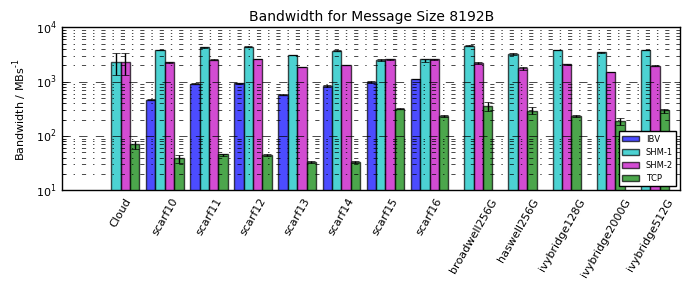
\includegraphics[width=\textwidth]{compare_bandwidth-hostgroup_8192}
      \caption{SCARF}
    \end{subfigure}

    \begin{subfigure}{\textwidth}
      \centering
        % This file was created by matplotlib2tikz v0.6.6.
\begin{tikzpicture}

\definecolor{color1}{rgb}{0.75,0,0.75}
\definecolor{color0}{rgb}{0,0.75,0.75}

\begin{axis}[
title={Bandwidth for Message Size 8192B},
ylabel={Bandwidth},
xmin=-1.74875, xmax=12.38625,
ymin=24.3351911340897, ymax=6009.34899562563,
ymode=log,
width=\figurewidth,
height=\figureheight,
xtick={-0.68125,0.31875,1.31875,2.31875,3.31875,4.31875,5.31875,6.31875,7.31875,8.31875,9.31875,10.31875,11.31875},
xticklabels={Cloud,scarf10,scarf11,scarf12,scarf13,scarf14,scarf15,scarf16,broadwell256G,haswell256G,ivybridge128G,ivybridge2000G,ivybridge512G},
ytick={1,10,100,1000,10000,100000},
yticklabels={,,${10^{2}}$,${10^{3}}$,,},
tick align=outside,
xticklabel style = {rotate=60},
xmajorticks=false,
ytick pos=left,
x grid style={white!69.019607843137251!black},
y grid style={white!69.019607843137251!black},
legend entries={{SHM-1},{TCP},{IBV},{SHM-2}},
legend style={at={(0.97,0.03)}, anchor=south east, draw=white!80.0!black},
legend cell align={left}
]
\addlegendimage{ybar,ybar legend,fill=color0,draw opacity=0};
\draw[fill=color0,draw opacity=0] (axis cs:-1.10625,0) rectangle (axis cs:-0.89375,2331.777);
\draw[fill=color0,draw opacity=0] (axis cs:-0.10625,0) rectangle (axis cs:0.10625,3786.752);
\draw[fill=color0,draw opacity=0] (axis cs:0.89375,0) rectangle (axis cs:1.10625,4266.714);
\draw[fill=color0,draw opacity=0] (axis cs:1.89375,0) rectangle (axis cs:2.10625,4399.958);
\draw[fill=color0,draw opacity=0] (axis cs:2.89375,0) rectangle (axis cs:3.10625,3153.468);
\draw[fill=color0,draw opacity=0] (axis cs:3.89375,0) rectangle (axis cs:4.10625,3735.094);
\draw[fill=color0,draw opacity=0] (axis cs:4.89375,0) rectangle (axis cs:5.10625,2513.02);
\draw[fill=color0,draw opacity=0] (axis cs:5.89375,0) rectangle (axis cs:6.10625,2566.256);
\draw[fill=color0,draw opacity=0] (axis cs:6.89375,0) rectangle (axis cs:7.10625,4615.698);
\draw[fill=color0,draw opacity=0] (axis cs:7.89375,0) rectangle (axis cs:8.10625,3248.41);
\draw[fill=color0,draw opacity=0] (axis cs:8.89375,0) rectangle (axis cs:9.10625,3794.902);
\draw[fill=color0,draw opacity=0] (axis cs:9.89375,0) rectangle (axis cs:10.10625,3479.324);
\draw[fill=color0,draw opacity=0] (axis cs:10.89375,0) rectangle (axis cs:11.10625,3784.998);
\addlegendimage{ybar,ybar legend,fill=green!50.0!black,draw opacity=0};
\draw[fill=green!50.0!black,draw opacity=0] (axis cs:-0.89375,0) rectangle (axis cs:-0.68125,70.8153333333333);
\draw[fill=green!50.0!black,draw opacity=0] (axis cs:0.10625,0) rectangle (axis cs:0.31875,39.924);
\draw[fill=green!50.0!black,draw opacity=0] (axis cs:1.10625,0) rectangle (axis cs:1.31875,45.962);
\draw[fill=green!50.0!black,draw opacity=0] (axis cs:2.10625,0) rectangle (axis cs:2.31875,45.632);
\draw[fill=green!50.0!black,draw opacity=0] (axis cs:3.10625,0) rectangle (axis cs:3.31875,32.814);
\draw[fill=green!50.0!black,draw opacity=0] (axis cs:4.10625,0) rectangle (axis cs:4.31875,33.336);
\draw[fill=green!50.0!black,draw opacity=0] (axis cs:5.10625,0) rectangle (axis cs:5.31875,318.38);
\draw[fill=green!50.0!black,draw opacity=0] (axis cs:6.10625,0) rectangle (axis cs:6.31875,233.964);
\draw[fill=green!50.0!black,draw opacity=0] (axis cs:7.10625,0) rectangle (axis cs:7.31875,352.734);
\draw[fill=green!50.0!black,draw opacity=0] (axis cs:8.10625,0) rectangle (axis cs:8.31875,289.126);
\draw[fill=green!50.0!black,draw opacity=0] (axis cs:9.10625,0) rectangle (axis cs:9.31875,235.512);
\draw[fill=green!50.0!black,draw opacity=0] (axis cs:10.10625,0) rectangle (axis cs:10.31875,188.944);
\draw[fill=green!50.0!black,draw opacity=0] (axis cs:11.10625,0) rectangle (axis cs:11.31875,295.25);
\addlegendimage{ybar,ybar legend,fill=blue,draw opacity=0};
\draw[fill=blue,draw opacity=0] (axis cs:-0.68125,0) rectangle (axis cs:-0.46875,0);
\draw[fill=blue,draw opacity=0] (axis cs:0.31875,0) rectangle (axis cs:0.53125,468.494);
\draw[fill=blue,draw opacity=0] (axis cs:1.31875,0) rectangle (axis cs:1.53125,913.838);
\draw[fill=blue,draw opacity=0] (axis cs:2.31875,0) rectangle (axis cs:2.53125,935.66);
\draw[fill=blue,draw opacity=0] (axis cs:3.31875,0) rectangle (axis cs:3.53125,579.114);
\draw[fill=blue,draw opacity=0] (axis cs:4.31875,0) rectangle (axis cs:4.53125,822.416);
\draw[fill=blue,draw opacity=0] (axis cs:5.31875,0) rectangle (axis cs:5.53125,988.264);
\draw[fill=blue,draw opacity=0] (axis cs:6.31875,0) rectangle (axis cs:6.53125,1122.512);
\draw[fill=blue,draw opacity=0] (axis cs:7.31875,0) rectangle (axis cs:7.53125,0);
\draw[fill=blue,draw opacity=0] (axis cs:8.31875,0) rectangle (axis cs:8.53125,0);
\draw[fill=blue,draw opacity=0] (axis cs:9.31875,0) rectangle (axis cs:9.53125,0);
\draw[fill=blue,draw opacity=0] (axis cs:10.31875,0) rectangle (axis cs:10.53125,0);
\draw[fill=blue,draw opacity=0] (axis cs:11.31875,0) rectangle (axis cs:11.53125,0);
\addlegendimage{ybar,ybar legend,fill=color1,draw opacity=0};
\draw[fill=color1,draw opacity=0] (axis cs:-0.46875,0) rectangle (axis cs:-0.25625,2331.777);
\draw[fill=color1,draw opacity=0] (axis cs:0.53125,0) rectangle (axis cs:0.74375,2269.976);
\draw[fill=color1,draw opacity=0] (axis cs:1.53125,0) rectangle (axis cs:1.74375,2559.634);
\draw[fill=color1,draw opacity=0] (axis cs:2.53125,0) rectangle (axis cs:2.74375,2601.344);
\draw[fill=color1,draw opacity=0] (axis cs:3.53125,0) rectangle (axis cs:3.74375,1891.894);
\draw[fill=color1,draw opacity=0] (axis cs:4.53125,0) rectangle (axis cs:4.74375,2005.548);
\draw[fill=color1,draw opacity=0] (axis cs:5.53125,0) rectangle (axis cs:5.74375,2563.464);
\draw[fill=color1,draw opacity=0] (axis cs:6.53125,0) rectangle (axis cs:6.74375,2568.836);
\draw[fill=color1,draw opacity=0] (axis cs:7.53125,0) rectangle (axis cs:7.74375,2204.372);
\draw[fill=color1,draw opacity=0] (axis cs:8.53125,0) rectangle (axis cs:8.74375,1752.092);
\draw[fill=color1,draw opacity=0] (axis cs:9.53125,0) rectangle (axis cs:9.74375,2106.112);
\draw[fill=color1,draw opacity=0] (axis cs:10.53125,0) rectangle (axis cs:10.74375,1514.618);
\draw[fill=color1,draw opacity=0] (axis cs:11.53125,0) rectangle (axis cs:11.74375,1983.108);
\path [draw=black, semithick] (axis cs:-1,1334.66)
--(axis cs:-1,3421.35);

\path [draw=black, semithick] (axis cs:0,3763.19)
--(axis cs:0,3822.01);

\path [draw=black, semithick] (axis cs:1,4227.58)
--(axis cs:1,4299.7);

\path [draw=black, semithick] (axis cs:2,4363.25)
--(axis cs:2,4446.43);

\path [draw=black, semithick] (axis cs:3,3125.67)
--(axis cs:3,3162.32);

\path [draw=black, semithick] (axis cs:4,3705.32)
--(axis cs:4,3787.99);

\path [draw=black, semithick] (axis cs:5,2363.87)
--(axis cs:5,2656.83);

\path [draw=black, semithick] (axis cs:6,2328.68)
--(axis cs:6,2663.2);

\path [draw=black, semithick] (axis cs:7,4543.54)
--(axis cs:7,4678.14);

\path [draw=black, semithick] (axis cs:8,3150.16)
--(axis cs:8,3318.78);

\path [draw=black, semithick] (axis cs:9,3768.6)
--(axis cs:9,3869.63);

\path [draw=black, semithick] (axis cs:10,3428.15)
--(axis cs:10,3520.79);

\path [draw=black, semithick] (axis cs:11,3755.21)
--(axis cs:11,3877.18);

\path [draw=black, semithick] (axis cs:-0.7875,58.13)
--(axis cs:-0.7875,82.72);

\path [draw=black, semithick] (axis cs:0.2125,31.26)
--(axis cs:0.2125,44.72);

\path [draw=black, semithick] (axis cs:1.2125,43.75)
--(axis cs:1.2125,47.48);

\path [draw=black, semithick] (axis cs:2.2125,43.77)
--(axis cs:2.2125,47.09);

\path [draw=black, semithick] (axis cs:3.2125,31.76)
--(axis cs:3.2125,34.03);

\path [draw=black, semithick] (axis cs:4.2125,32.17)
--(axis cs:4.2125,34.61);

\path [draw=black, semithick] (axis cs:5.2125,311.32)
--(axis cs:5.2125,322.93);

\path [draw=black, semithick] (axis cs:6.2125,221.94)
--(axis cs:6.2125,244.81);

\path [draw=black, semithick] (axis cs:7.2125,293.37)
--(axis cs:7.2125,421.93);

\path [draw=black, semithick] (axis cs:8.2125,257.29)
--(axis cs:8.2125,337.83);

\path [draw=black, semithick] (axis cs:9.2125,225.96)
--(axis cs:9.2125,247.97);

\path [draw=black, semithick] (axis cs:10.2125,158.3)
--(axis cs:10.2125,210.96);

\path [draw=black, semithick] (axis cs:11.2125,266.01)
--(axis cs:11.2125,320.65);

\path [draw=black, semithick] (axis cs:-0.575,0)
--(axis cs:-0.575,0);

\path [draw=black, semithick] (axis cs:0.425,465.9)
--(axis cs:0.425,472.75);

\path [draw=black, semithick] (axis cs:1.425,903.28)
--(axis cs:1.425,929.73);

\path [draw=black, semithick] (axis cs:2.425,924.5)
--(axis cs:2.425,952.52);

\path [draw=black, semithick] (axis cs:3.425,564.18)
--(axis cs:3.425,595.31);

\path [draw=black, semithick] (axis cs:4.425,807.87)
--(axis cs:4.425,862.41);

\path [draw=black, semithick] (axis cs:5.425,937.03)
--(axis cs:5.425,1016.2);

\path [draw=black, semithick] (axis cs:6.425,1114.48)
--(axis cs:6.425,1129.64);

\path [draw=black, semithick] (axis cs:7.425,0)
--(axis cs:7.425,0);

\path [draw=black, semithick] (axis cs:8.425,0)
--(axis cs:8.425,0);

\path [draw=black, semithick] (axis cs:9.425,0)
--(axis cs:9.425,0);

\path [draw=black, semithick] (axis cs:10.425,0)
--(axis cs:10.425,0);

\path [draw=black, semithick] (axis cs:11.425,0)
--(axis cs:11.425,0);

\path [draw=black, semithick] (axis cs:-0.3625,1334.66)
--(axis cs:-0.3625,3421.35);

\path [draw=black, semithick] (axis cs:0.6375,2234.44)
--(axis cs:0.6375,2303.87);

\path [draw=black, semithick] (axis cs:1.6375,2529.08)
--(axis cs:1.6375,2603.32);

\path [draw=black, semithick] (axis cs:2.6375,2589.03)
--(axis cs:2.6375,2624.8);

\path [draw=black, semithick] (axis cs:3.6375,1880.03)
--(axis cs:3.6375,1898.55);

\path [draw=black, semithick] (axis cs:4.6375,1998.84)
--(axis cs:4.6375,2014.32);

\path [draw=black, semithick] (axis cs:5.6375,2493.19)
--(axis cs:5.6375,2587.8);

\path [draw=black, semithick] (axis cs:6.6375,2539.86)
--(axis cs:6.6375,2582.29);

\path [draw=black, semithick] (axis cs:7.6375,2143.94)
--(axis cs:7.6375,2306.31);

\path [draw=black, semithick] (axis cs:8.6375,1633.74)
--(axis cs:8.6375,1832.87);

\path [draw=black, semithick] (axis cs:9.6375,2054.03)
--(axis cs:9.6375,2131.04);

\path [draw=black, semithick] (axis cs:10.6375,1496.63)
--(axis cs:10.6375,1532.04);

\path [draw=black, semithick] (axis cs:11.6375,1933.1)
--(axis cs:11.6375,2022.65);

\addplot [semithick, black]
table {%
-1 2331.777
0 3786.752
1 4266.714
2 4399.958
3 3153.468
4 3735.094
5 2513.02
6 2566.256
7 4615.698
8 3248.41
9 3794.902
10 3479.324
11 3784.998
};
\addplot [semithick, black]
table {%
-0.7875 70.8153333333333
0.2125 39.924
1.2125 45.962
2.2125 45.632
3.2125 32.814
4.2125 33.336
5.2125 318.38
6.2125 233.964
7.2125 352.734
8.2125 289.126
9.2125 235.512
10.2125 188.944
11.2125 295.25
};
\addplot [semithick, black]
table {%
-0.575 0
0.425 468.494
1.425 913.838
2.425 935.66
3.425 579.114
4.425 822.416
5.425 988.264
6.425 1122.512
7.425 0
8.425 0
9.425 0
10.425 0
11.425 0
};
\addplot [semithick, black]
table {%
-0.3625 2331.777
0.6375 2269.976
1.6375 2559.634
2.6375 2601.344
3.6375 1891.894
4.6375 2005.548
5.6375 2563.464
6.6375 2568.836
7.6375 2204.372
8.6375 1752.092
9.6375 2106.112
10.6375 1514.618
11.6375 1983.108
};
\end{axis}

\end{tikzpicture}
    %   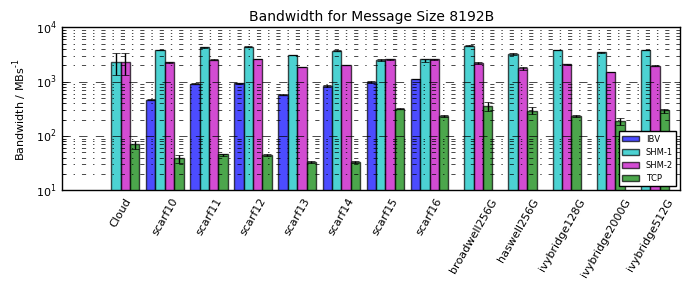
\includegraphics[width=\textwidth]{compare_bandwidth-hostgroup_8192}
      \caption{LOTUS}
    \end{subfigure}
    \caption{OVERALL CAPTION (halfway)}
 \end{figure}

 \begin{figure}[H]\ContinuedFloat
    \centering
    \begin{subfigure}{\textwidth}
      \centering
        % This file was created by matplotlib2tikz v0.6.6.
\begin{tikzpicture}

\definecolor{color1}{rgb}{0,0.75,0.75}
\definecolor{color0}{rgb}{0.75,0,0.75}

\begin{axis}[
title={Bandwidth for Message Size 32768B},
ylabel={Bandwidth \si{\mega\byte\per\second}},
xmin=-1.74875, xmax=12.38625,
ymin=20.5819620180395, ymax=9490.59996460947,
ymode=log,
width=\figurewidth,
height=\figureheight,
xtick={-0.68125,0.31875,1.31875,2.31875,3.31875,4.31875,5.31875,6.31875,7.31875,8.31875,9.31875,10.31875,11.31875},
xticklabels={Cloud,scarf10,scarf11,scarf12,scarf13,scarf14,scarf15,scarf16,broadwell256G,haswell256G,ivybridge128G,ivybridge2000G,ivybridge512G},
ytick={1,10,100,1000,10000,100000},
yticklabels={,,${10^{2}}$,${10^{3}}$,,},
tick align=outside,
xticklabel style = {rotate=60},
xmajorticks=false,
ytick pos=left,
x grid style={lightgray!92.026143790849673!black},
y grid style={lightgray!92.026143790849673!black},
legend style={at={(0.97,0.03)}, anchor=south east, draw=white!80.0!black},
legend entries={{IBV},{SHM-2},{SHM-1},{TCP}},
legend cell align={left}
]
\addlegendimage{ybar,ybar legend,fill=blue,draw opacity=0};
\draw[fill=blue,draw opacity=0] (axis cs:-1.10625,0) rectangle (axis cs:-0.89375,0);
\draw[fill=blue,draw opacity=0] (axis cs:-0.10625,0) rectangle (axis cs:0.10625,654.378);
\draw[fill=blue,draw opacity=0] (axis cs:0.89375,0) rectangle (axis cs:1.10625,1699.7);
\draw[fill=blue,draw opacity=0] (axis cs:1.89375,0) rectangle (axis cs:2.10625,1743.982);
\draw[fill=blue,draw opacity=0] (axis cs:2.89375,0) rectangle (axis cs:3.10625,747.124);
\draw[fill=blue,draw opacity=0] (axis cs:3.89375,0) rectangle (axis cs:4.10625,1796.934);
\draw[fill=blue,draw opacity=0] (axis cs:4.89375,0) rectangle (axis cs:5.10625,2308.61);
\draw[fill=blue,draw opacity=0] (axis cs:5.89375,0) rectangle (axis cs:6.10625,2702.852);
\draw[fill=blue,draw opacity=0] (axis cs:6.89375,0) rectangle (axis cs:7.10625,0);
\draw[fill=blue,draw opacity=0] (axis cs:7.89375,0) rectangle (axis cs:8.10625,0);
\draw[fill=blue,draw opacity=0] (axis cs:8.89375,0) rectangle (axis cs:9.10625,0);
\draw[fill=blue,draw opacity=0] (axis cs:9.89375,0) rectangle (axis cs:10.10625,0);
\draw[fill=blue,draw opacity=0] (axis cs:10.89375,0) rectangle (axis cs:11.10625,0);
\addlegendimage{ybar,ybar legend,fill=color0,draw opacity=0};
\draw[fill=color0,draw opacity=0] (axis cs:-0.89375,0) rectangle (axis cs:-0.68125,3164.25766666667);
\draw[fill=color0,draw opacity=0] (axis cs:0.10625,0) rectangle (axis cs:0.31875,3478.144);
\draw[fill=color0,draw opacity=0] (axis cs:1.10625,0) rectangle (axis cs:1.31875,3879.78);
\draw[fill=color0,draw opacity=0] (axis cs:2.10625,0) rectangle (axis cs:2.31875,3952.472);
\draw[fill=color0,draw opacity=0] (axis cs:3.10625,0) rectangle (axis cs:3.31875,2841.634);
\draw[fill=color0,draw opacity=0] (axis cs:4.10625,0) rectangle (axis cs:4.31875,2931.54);
\draw[fill=color0,draw opacity=0] (axis cs:5.10625,0) rectangle (axis cs:5.31875,3905.398);
\draw[fill=color0,draw opacity=0] (axis cs:6.10625,0) rectangle (axis cs:6.31875,3881.204);
\draw[fill=color0,draw opacity=0] (axis cs:7.10625,0) rectangle (axis cs:7.31875,3160.148);
\draw[fill=color0,draw opacity=0] (axis cs:8.10625,0) rectangle (axis cs:8.31875,2633.924);
\draw[fill=color0,draw opacity=0] (axis cs:9.10625,0) rectangle (axis cs:9.31875,3041.108);
\draw[fill=color0,draw opacity=0] (axis cs:10.10625,0) rectangle (axis cs:10.31875,1968.708);
\draw[fill=color0,draw opacity=0] (axis cs:11.10625,0) rectangle (axis cs:11.31875,2946.584);
\addlegendimage{ybar,ybar legend,fill=color1,draw opacity=0};
\draw[fill=color1,draw opacity=0] (axis cs:-0.68125,0) rectangle (axis cs:-0.46875,3164.25766666667);
\draw[fill=color1,draw opacity=0] (axis cs:0.31875,0) rectangle (axis cs:0.53125,5432.64);
\draw[fill=color1,draw opacity=0] (axis cs:1.31875,0) rectangle (axis cs:1.53125,6071.522);
\draw[fill=color1,draw opacity=0] (axis cs:2.31875,0) rectangle (axis cs:2.53125,6503.346);
\draw[fill=color1,draw opacity=0] (axis cs:3.31875,0) rectangle (axis cs:3.53125,4854.996);
\draw[fill=color1,draw opacity=0] (axis cs:4.31875,0) rectangle (axis cs:4.53125,5775.772);
\draw[fill=color1,draw opacity=0] (axis cs:5.31875,0) rectangle (axis cs:5.53125,3486.676);
\draw[fill=color1,draw opacity=0] (axis cs:6.31875,0) rectangle (axis cs:6.53125,3473.624);
\draw[fill=color1,draw opacity=0] (axis cs:7.31875,0) rectangle (axis cs:7.53125,7150.788);
\draw[fill=color1,draw opacity=0] (axis cs:8.31875,0) rectangle (axis cs:8.53125,4872.268);
\draw[fill=color1,draw opacity=0] (axis cs:9.31875,0) rectangle (axis cs:9.53125,6045.878);
\draw[fill=color1,draw opacity=0] (axis cs:10.31875,0) rectangle (axis cs:10.53125,5605.092);
\draw[fill=color1,draw opacity=0] (axis cs:11.31875,0) rectangle (axis cs:11.53125,6033.936);
\addlegendimage{ybar,ybar legend,fill=green!50.0!black,draw opacity=0};
\draw[fill=green!50.0!black,draw opacity=0] (axis cs:-0.46875,0) rectangle (axis cs:-0.25625,184.263333333333);
\draw[fill=green!50.0!black,draw opacity=0] (axis cs:0.53125,0) rectangle (axis cs:0.74375,34.994);
\draw[fill=green!50.0!black,draw opacity=0] (axis cs:1.53125,0) rectangle (axis cs:1.74375,48.05);
\draw[fill=green!50.0!black,draw opacity=0] (axis cs:2.53125,0) rectangle (axis cs:2.74375,40.03);
\draw[fill=green!50.0!black,draw opacity=0] (axis cs:3.53125,0) rectangle (axis cs:3.74375,55.674);
\draw[fill=green!50.0!black,draw opacity=0] (axis cs:4.53125,0) rectangle (axis cs:4.74375,56.766);
\draw[fill=green!50.0!black,draw opacity=0] (axis cs:5.53125,0) rectangle (axis cs:5.74375,463.962);
\draw[fill=green!50.0!black,draw opacity=0] (axis cs:6.53125,0) rectangle (axis cs:6.74375,342.794);
\draw[fill=green!50.0!black,draw opacity=0] (axis cs:7.53125,0) rectangle (axis cs:7.74375,502.72);
\draw[fill=green!50.0!black,draw opacity=0] (axis cs:8.53125,0) rectangle (axis cs:8.74375,409.642);
\draw[fill=green!50.0!black,draw opacity=0] (axis cs:9.53125,0) rectangle (axis cs:9.74375,371.358);
\draw[fill=green!50.0!black,draw opacity=0] (axis cs:10.53125,0) rectangle (axis cs:10.74375,311.786);
\draw[fill=green!50.0!black,draw opacity=0] (axis cs:11.53125,0) rectangle (axis cs:11.74375,429.372);
\path [draw=black, semithick] (axis cs:-1,0)
--(axis cs:-1,0);

\path [draw=black, semithick] (axis cs:0,651.48)
--(axis cs:0,656.11);

\path [draw=black, semithick] (axis cs:1,1675.78)
--(axis cs:1,1733.94);

\path [draw=black, semithick] (axis cs:2,1733.23)
--(axis cs:2,1756.86);

\path [draw=black, semithick] (axis cs:3,716.66)
--(axis cs:3,770.82);

\path [draw=black, semithick] (axis cs:4,1645.47)
--(axis cs:4,1965.29);

\path [draw=black, semithick] (axis cs:5,2078)
--(axis cs:5,2431.9);

\path [draw=black, semithick] (axis cs:6,2680.57)
--(axis cs:6,2715.48);

\path [draw=black, semithick] (axis cs:7,0)
--(axis cs:7,0);

\path [draw=black, semithick] (axis cs:8,0)
--(axis cs:8,0);

\path [draw=black, semithick] (axis cs:9,0)
--(axis cs:9,0);

\path [draw=black, semithick] (axis cs:10,0)
--(axis cs:10,0);

\path [draw=black, semithick] (axis cs:11,0)
--(axis cs:11,0);

\path [draw=black, semithick] (axis cs:-0.7875,1716.7)
--(axis cs:-0.7875,4404.52);

\path [draw=black, semithick] (axis cs:0.2125,3409.16)
--(axis cs:0.2125,3539.28);

\path [draw=black, semithick] (axis cs:1.2125,3828.48)
--(axis cs:1.2125,3935.27);

\path [draw=black, semithick] (axis cs:2.2125,3927.31)
--(axis cs:2.2125,3972.3);

\path [draw=black, semithick] (axis cs:3.2125,2824.34)
--(axis cs:3.2125,2853.36);

\path [draw=black, semithick] (axis cs:4.2125,2904.96)
--(axis cs:4.2125,2944.64);

\path [draw=black, semithick] (axis cs:5.2125,3787.88)
--(axis cs:5.2125,3964.97);

\path [draw=black, semithick] (axis cs:6.2125,3800.07)
--(axis cs:6.2125,3974.05);

\path [draw=black, semithick] (axis cs:7.2125,3149.9)
--(axis cs:7.2125,3176.46);

\path [draw=black, semithick] (axis cs:8.2125,2608.5)
--(axis cs:8.2125,2662.77);

\path [draw=black, semithick] (axis cs:9.2125,3028.85)
--(axis cs:9.2125,3054.9);

\path [draw=black, semithick] (axis cs:10.2125,1944.01)
--(axis cs:10.2125,1981.48);

\path [draw=black, semithick] (axis cs:11.2125,2861.05)
--(axis cs:11.2125,2988.72);

\path [draw=black, semithick] (axis cs:-0.575,1716.7)
--(axis cs:-0.575,4404.52);

\path [draw=black, semithick] (axis cs:0.425,5386.59)
--(axis cs:0.425,5508.5);

\path [draw=black, semithick] (axis cs:1.425,5996.39)
--(axis cs:1.425,6201.66);

\path [draw=black, semithick] (axis cs:2.425,6423.37)
--(axis cs:2.425,6610.28);

\path [draw=black, semithick] (axis cs:3.425,4810.6)
--(axis cs:3.425,4898.51);

\path [draw=black, semithick] (axis cs:4.425,5736.07)
--(axis cs:4.425,5821.02);

\path [draw=black, semithick] (axis cs:5.425,3430.89)
--(axis cs:5.425,3573.44);

\path [draw=black, semithick] (axis cs:6.425,3410.27)
--(axis cs:6.425,3516.35);

\path [draw=black, semithick] (axis cs:7.425,7103.02)
--(axis cs:7.425,7181.44);

\path [draw=black, semithick] (axis cs:8.425,4790.73)
--(axis cs:8.425,4976.16);

\path [draw=black, semithick] (axis cs:9.425,5931.4)
--(axis cs:9.425,6117.28);

\path [draw=black, semithick] (axis cs:10.425,5486.25)
--(axis cs:10.425,5685.43);

\path [draw=black, semithick] (axis cs:11.425,5999.68)
--(axis cs:11.425,6099.92);

\path [draw=black, semithick] (axis cs:-0.3625,153.11)
--(axis cs:-0.3625,213.42);

\path [draw=black, semithick] (axis cs:0.6375,27.2)
--(axis cs:0.6375,44.24);

\path [draw=black, semithick] (axis cs:1.6375,45.78)
--(axis cs:1.6375,53.27);

\path [draw=black, semithick] (axis cs:2.6375,36.1)
--(axis cs:2.6375,42.36);

\path [draw=black, semithick] (axis cs:3.6375,52.05)
--(axis cs:3.6375,57.37);

\path [draw=black, semithick] (axis cs:4.6375,53.29)
--(axis cs:4.6375,57.74);

\path [draw=black, semithick] (axis cs:5.6375,459.03)
--(axis cs:5.6375,467.1);

\path [draw=black, semithick] (axis cs:6.6375,322.23)
--(axis cs:6.6375,372.99);

\path [draw=black, semithick] (axis cs:7.6375,451.47)
--(axis cs:7.6375,566.39);

\path [draw=black, semithick] (axis cs:8.6375,374.29)
--(axis cs:8.6375,463.05);

\path [draw=black, semithick] (axis cs:9.6375,353.04)
--(axis cs:9.6375,396.35);

\path [draw=black, semithick] (axis cs:10.6375,262.23)
--(axis cs:10.6375,340.78);

\path [draw=black, semithick] (axis cs:11.6375,376)
--(axis cs:11.6375,468.28);

\end{axis}

\end{tikzpicture}
    %   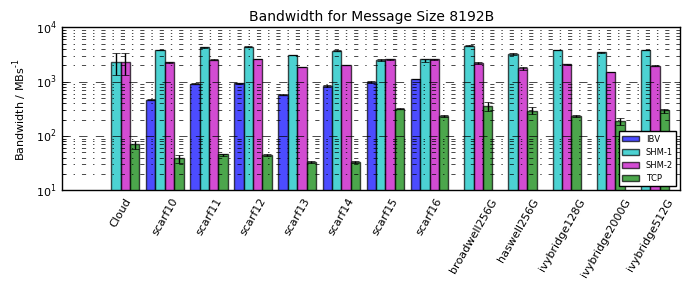
\includegraphics[width=\textwidth]{compare_bandwidth-hostgroup_8192}
      \caption{SCARF}
    \end{subfigure}

    \begin{subfigure}{\textwidth}
      \centering
        % This file was created by matplotlib2tikz v0.6.6.
\begin{tikzpicture}

\definecolor{color1}{rgb}{0,0.75,0.75}
\definecolor{color0}{rgb}{0.75,0,0.75}

\begin{axis}[
title={Max Bandwidth},
ylabel={Max Bandwidth},
xmin=-1.74875, xmax=12.38625,
ymin=10, ymax=100000,
ymode=log,
width=\figurewidth,
height=\figureheight,
xtick={-0.68125,0.31875,1.31875,2.31875,3.31875,4.31875,5.31875,6.31875,7.31875,8.31875,9.31875,10.31875,11.31875},
xticklabels={Cloud,scarf10,scarf11,scarf12,scarf13,scarf14,scarf15,scarf16,broadwell256G,haswell256G,ivybridge128G,ivybridge2000G,ivybridge512G},
ytick={1,10,100,1000,10000,100000,1000000},
yticklabels={,,${10^{2}}$,${10^{3}}$,${10^{4}}$,,},
tick align=outside,
xticklabel style = {rotate=60},
xmajorticks=false,
ytick pos=left,
x grid style={lightgray!92.026143790849673!black},
y grid style={lightgray!92.026143790849673!black},
legend style={at={(0.97,0.03)}, anchor=south east, draw=white!80.0!black},
legend entries={{IBV},{SHM-2},{SHM-1},{TCP}},
legend cell align={left}
]
\addlegendimage{ybar,ybar legend,fill=blue,draw opacity=0};
\draw[fill=blue,draw opacity=0] (axis cs:-1.10625,0) rectangle (axis cs:-0.89375,0);
\draw[fill=blue,draw opacity=0] (axis cs:-0.10625,0) rectangle (axis cs:0.10625,1270.664);
\draw[fill=blue,draw opacity=0] (axis cs:0.89375,0) rectangle (axis cs:1.10625,3215.99);
\draw[fill=blue,draw opacity=0] (axis cs:1.89375,0) rectangle (axis cs:2.10625,3207.532);
\draw[fill=blue,draw opacity=0] (axis cs:2.89375,0) rectangle (axis cs:3.10625,2940.256);
\draw[fill=blue,draw opacity=0] (axis cs:3.89375,0) rectangle (axis cs:4.10625,3267.558);
\draw[fill=blue,draw opacity=0] (axis cs:4.89375,0) rectangle (axis cs:5.10625,5670.066);
\draw[fill=blue,draw opacity=0] (axis cs:5.89375,0) rectangle (axis cs:6.10625,5975.284);
\draw[fill=blue,draw opacity=0] (axis cs:6.89375,0) rectangle (axis cs:7.10625,0);
\draw[fill=blue,draw opacity=0] (axis cs:7.89375,0) rectangle (axis cs:8.10625,0);
\draw[fill=blue,draw opacity=0] (axis cs:8.89375,0) rectangle (axis cs:9.10625,0);
\draw[fill=blue,draw opacity=0] (axis cs:9.89375,0) rectangle (axis cs:10.10625,0);
\draw[fill=blue,draw opacity=0] (axis cs:10.89375,0) rectangle (axis cs:11.10625,0);
\addlegendimage{ybar,ybar legend,fill=color0,draw opacity=0};
\draw[fill=color0,draw opacity=0] (axis cs:-0.89375,0) rectangle (axis cs:-0.68125,6504.27033333333);
\draw[fill=color0,draw opacity=0] (axis cs:0.10625,0) rectangle (axis cs:0.31875,5048.188);
\draw[fill=color0,draw opacity=0] (axis cs:1.10625,0) rectangle (axis cs:1.31875,6974.272);
\draw[fill=color0,draw opacity=0] (axis cs:2.10625,0) rectangle (axis cs:2.31875,5787.316);
\draw[fill=color0,draw opacity=0] (axis cs:3.10625,0) rectangle (axis cs:3.31875,3927.28);
\draw[fill=color0,draw opacity=0] (axis cs:4.10625,0) rectangle (axis cs:4.31875,3973.648);
\draw[fill=color0,draw opacity=0] (axis cs:5.10625,0) rectangle (axis cs:5.31875,5876.906);
\draw[fill=color0,draw opacity=0] (axis cs:6.10625,0) rectangle (axis cs:6.31875,5905.492);
\draw[fill=color0,draw opacity=0] (axis cs:7.10625,0) rectangle (axis cs:7.31875,5920.182);
\draw[fill=color0,draw opacity=0] (axis cs:8.10625,0) rectangle (axis cs:8.31875,5006.572);
\draw[fill=color0,draw opacity=0] (axis cs:9.10625,0) rectangle (axis cs:9.31875,4299.586);
\draw[fill=color0,draw opacity=0] (axis cs:10.10625,0) rectangle (axis cs:10.31875,2417.754);
\draw[fill=color0,draw opacity=0] (axis cs:11.10625,0) rectangle (axis cs:11.31875,4167.016);
\addlegendimage{ybar,ybar legend,fill=color1,draw opacity=0};
\draw[fill=color1,draw opacity=0] (axis cs:-0.68125,0) rectangle (axis cs:-0.46875,6504.27033333333);
\draw[fill=color1,draw opacity=0] (axis cs:0.31875,0) rectangle (axis cs:0.53125,7419.946);
\draw[fill=color1,draw opacity=0] (axis cs:1.31875,0) rectangle (axis cs:1.53125,8877.112);
\draw[fill=color1,draw opacity=0] (axis cs:2.31875,0) rectangle (axis cs:2.53125,9121.696);
\draw[fill=color1,draw opacity=0] (axis cs:3.31875,0) rectangle (axis cs:3.53125,7504.84);
\draw[fill=color1,draw opacity=0] (axis cs:4.31875,0) rectangle (axis cs:4.53125,9153.448);
\draw[fill=color1,draw opacity=0] (axis cs:5.31875,0) rectangle (axis cs:5.53125,5145.8);
\draw[fill=color1,draw opacity=0] (axis cs:6.31875,0) rectangle (axis cs:6.53125,5140.572);
\draw[fill=color1,draw opacity=0] (axis cs:7.31875,0) rectangle (axis cs:7.53125,11468.012);
\draw[fill=color1,draw opacity=0] (axis cs:8.31875,0) rectangle (axis cs:8.53125,7683.796);
\draw[fill=color1,draw opacity=0] (axis cs:9.31875,0) rectangle (axis cs:9.53125,9115.23);
\draw[fill=color1,draw opacity=0] (axis cs:10.31875,0) rectangle (axis cs:10.53125,7808.318);
\draw[fill=color1,draw opacity=0] (axis cs:11.31875,0) rectangle (axis cs:11.53125,9082.176);
\addlegendimage{ybar,ybar legend,fill=green!50.0!black,draw opacity=0};
\draw[fill=green!50.0!black,draw opacity=0] (axis cs:-0.46875,0) rectangle (axis cs:-0.25625,456.419333333333);
\draw[fill=green!50.0!black,draw opacity=0] (axis cs:0.53125,0) rectangle (axis cs:0.74375,101.542);
\draw[fill=green!50.0!black,draw opacity=0] (axis cs:1.53125,0) rectangle (axis cs:1.74375,103.09);
\draw[fill=green!50.0!black,draw opacity=0] (axis cs:2.53125,0) rectangle (axis cs:2.74375,102.912);
\draw[fill=green!50.0!black,draw opacity=0] (axis cs:3.53125,0) rectangle (axis cs:3.74375,110.512);
\draw[fill=green!50.0!black,draw opacity=0] (axis cs:4.53125,0) rectangle (axis cs:4.74375,111.814);
\draw[fill=green!50.0!black,draw opacity=0] (axis cs:5.53125,0) rectangle (axis cs:5.74375,825.884);
\draw[fill=green!50.0!black,draw opacity=0] (axis cs:6.53125,0) rectangle (axis cs:6.74375,934.164);
\draw[fill=green!50.0!black,draw opacity=0] (axis cs:7.53125,0) rectangle (axis cs:7.74375,1174.91);
\draw[fill=green!50.0!black,draw opacity=0] (axis cs:8.53125,0) rectangle (axis cs:8.74375,1171.086);
\draw[fill=green!50.0!black,draw opacity=0] (axis cs:9.53125,0) rectangle (axis cs:9.74375,1172.704);
\draw[fill=green!50.0!black,draw opacity=0] (axis cs:10.53125,0) rectangle (axis cs:10.74375,1163.616);
\draw[fill=green!50.0!black,draw opacity=0] (axis cs:11.53125,0) rectangle (axis cs:11.74375,1172.762);
\path [draw=black, semithick] (axis cs:-1,0)
--(axis cs:-1,0);

\path [draw=black, semithick] (axis cs:0,1230.24)
--(axis cs:0,1331.43);

\path [draw=black, semithick] (axis cs:1,3202.46)
--(axis cs:1,3220.18);

\path [draw=black, semithick] (axis cs:2,3203.95)
--(axis cs:2,3220.02);

\path [draw=black, semithick] (axis cs:3,2738.79)
--(axis cs:3,3192.06);

\path [draw=black, semithick] (axis cs:4,3005.72)
--(axis cs:4,3602.61);

\path [draw=black, semithick] (axis cs:5,4986.63)
--(axis cs:5,5964.12);

\path [draw=black, semithick] (axis cs:6,5969.14)
--(axis cs:6,5979.33);

\path [draw=black, semithick] (axis cs:7,0)
--(axis cs:7,0);

\path [draw=black, semithick] (axis cs:8,0)
--(axis cs:8,0);

\path [draw=black, semithick] (axis cs:9,0)
--(axis cs:9,0);

\path [draw=black, semithick] (axis cs:10,0)
--(axis cs:10,0);

\path [draw=black, semithick] (axis cs:11,0)
--(axis cs:11,0);

\path [draw=black, semithick] (axis cs:-0.7875,3524.63)
--(axis cs:-0.7875,7717.49);

\path [draw=black, semithick] (axis cs:0.2125,5032.47)
--(axis cs:0.2125,5077.66);

\path [draw=black, semithick] (axis cs:1.2125,5690.98)
--(axis cs:1.2125,8316.65);

\path [draw=black, semithick] (axis cs:2.2125,5745.05)
--(axis cs:2.2125,5839.48);

\path [draw=black, semithick] (axis cs:3.2125,3915.63)
--(axis cs:3.2125,3934.26);

\path [draw=black, semithick] (axis cs:4.2125,3962.43)
--(axis cs:4.2125,3983.97);

\path [draw=black, semithick] (axis cs:5.2125,5860.33)
--(axis cs:5.2125,5909.22);

\path [draw=black, semithick] (axis cs:6.2125,5870.66)
--(axis cs:6.2125,5960.74);

\path [draw=black, semithick] (axis cs:7.2125,5810.72)
--(axis cs:7.2125,5965.29);

\path [draw=black, semithick] (axis cs:8.2125,4980.57)
--(axis cs:8.2125,5043.61);

\path [draw=black, semithick] (axis cs:9.2125,4294.96)
--(axis cs:9.2125,4305.48);

\path [draw=black, semithick] (axis cs:10.2125,2394.88)
--(axis cs:10.2125,2429.22);

\path [draw=black, semithick] (axis cs:11.2125,4137.07)
--(axis cs:11.2125,4197.83);

\path [draw=black, semithick] (axis cs:-0.575,3524.63)
--(axis cs:-0.575,7717.49);

\path [draw=black, semithick] (axis cs:0.425,7336.75)
--(axis cs:0.425,7502.58);

\path [draw=black, semithick] (axis cs:1.425,8836.15)
--(axis cs:1.425,8928.33);

\path [draw=black, semithick] (axis cs:2.425,8984.73)
--(axis cs:2.425,9256.52);

\path [draw=black, semithick] (axis cs:3.425,7472.36)
--(axis cs:3.425,7526.92);

\path [draw=black, semithick] (axis cs:4.425,9123.55)
--(axis cs:4.425,9184.85);

\path [draw=black, semithick] (axis cs:5.425,5126.21)
--(axis cs:5.425,5177.6);

\path [draw=black, semithick] (axis cs:6.425,5055.94)
--(axis cs:6.425,5213.28);

\path [draw=black, semithick] (axis cs:7.425,11365.12)
--(axis cs:7.425,11564);

\path [draw=black, semithick] (axis cs:8.425,7334.57)
--(axis cs:8.425,7971.05);

\path [draw=black, semithick] (axis cs:9.425,9053.32)
--(axis cs:9.425,9176.5);

\path [draw=black, semithick] (axis cs:10.425,7726.6)
--(axis cs:10.425,7867.15);

\path [draw=black, semithick] (axis cs:11.425,8940.91)
--(axis cs:11.425,9150.76);

\path [draw=black, semithick] (axis cs:-0.3625,406.85)
--(axis cs:-0.3625,506.17);

\path [draw=black, semithick] (axis cs:0.6375,100.61)
--(axis cs:0.6375,103.26);

\path [draw=black, semithick] (axis cs:1.6375,101.46)
--(axis cs:1.6375,105.62);

\path [draw=black, semithick] (axis cs:2.6375,102.18)
--(axis cs:2.6375,103.54);

\path [draw=black, semithick] (axis cs:3.6375,109.84)
--(axis cs:3.6375,110.98);

\path [draw=black, semithick] (axis cs:4.6375,111.31)
--(axis cs:4.6375,111.95);

\path [draw=black, semithick] (axis cs:5.6375,813.51)
--(axis cs:5.6375,861.5);

\path [draw=black, semithick] (axis cs:6.6375,917.64)
--(axis cs:6.6375,951.98);

\path [draw=black, semithick] (axis cs:7.6375,1174.33)
--(axis cs:7.6375,1175.82);

\path [draw=black, semithick] (axis cs:8.6375,1169.82)
--(axis cs:8.6375,1172.1);

\path [draw=black, semithick] (axis cs:9.6375,1172.1)
--(axis cs:9.6375,1172.94);

\path [draw=black, semithick] (axis cs:10.6375,1158.17)
--(axis cs:10.6375,1168.5);

\path [draw=black, semithick] (axis cs:11.6375,1172.31)
--(axis cs:11.6375,1173.26);

\end{axis}

\end{tikzpicture}
    %   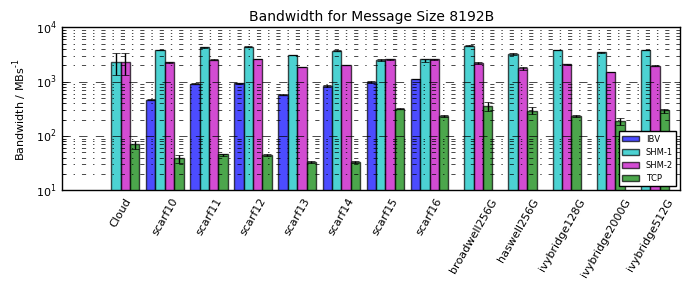
\includegraphics[width=\textwidth]{compare_bandwidth-hostgroup_8192}
      \caption{LOTUS}
    \end{subfigure}
    \caption{OVERALL CAPTION (halfway)}
 \end{figure}
\end{landscape}


\end{document}
